\section{Wprowadzenie}
    \subsection{Cel ćwiczenia}
        Celem ćwiczenia było poznanie tzw. naiwnego klasyfikatora Bayesa oraz zbadanie i ocena jego
        działania na 3 określonych zbiorach danych. W trakcie badań należało uwzględnić różne metody
        dyskretyzacji danych i kroswalidacji oraz zaobserwować wpływ tych parametrów na wartości
        zadanych metryk.

    \subsection{Klasyfikator Bayesowski}
        Typowym zagadnieniem w uczeniu maszynowym jest zadanie klasyfikacji. Należy ono do grupy
        tzw. \textbf{zadań uczenia nadzorowanego}, czyli zakłada istnienie zbioru danych, w którym każda
        instancja (wektor cech) jest oznaczona odpowiednią etykietą (\textit{klasa}). Narzędzie, które
        jest uczone na takim zbiorze, a następnie używane do przyporządkowywania etykiet do nowych
        instancji, nazywa się \textbf{klasyfikatorem}. W tym ćwiczeniu użyty zostanie \textbf{naiwny klasyfikator
        Bayesowski} (ang. \textit{Naive Bayes Classifier}). Jest on oparty o twierdzenie Bayesa:

        $$ P(Y | X ) = \frac{P(X|Y)P(Y)}{P(X)}$$

        \noindent gdzie: \\
        \textbf{X} - wektor cech danej instancji, \\
        \textbf{Y} - klasa.\\

        \noindent Powyższy zapis odczytujemy jako prawdopodobieństwo przynależności instancji X do klasy Y.
        Ważne jest, że ten klasyfikator zakłada niezależność wszystkich atrybutów (cech), co w większości przypadków
        się nie sprawdza (stąd nazwa \textit{naiwny}). Stąd w powyższym wzorze, człon $P(X|Y)$ można zastąpić iloczynem
        prawdopodobieństw:
            $$ P(X|Y) = \prod_{i= 1}^{n}P(X_i|Y)$$

        \noindent Problem jaki się tutaj pojawia, to sytuacja w której jedno z prawdopodobieństw $P(X_i|Y) = 0$, wtedy cały
        iloczyn się również wyzeruje. W celu przecidziałania temu, stosuje się tzw. wygładzanie danych -- dla metody Laplace'a
        zwiększa się częstość występowania danego atrybutu. Klasa przypisywana przez klasyfikator dla danej instancji jest
        dobierana w taki sposób, aby prawdopodobieństwo $P(Y|X)$ przyjęło największą sposród możliwych wartości.
        \vspace{1em}

        \noindent Można wyróżnić 2 główne typy klasyfikatorów Bayesowskich:
        \begin{itemize}
            \item{\textbf{Gaussowski naiwny Bayes} -- atrybuty przyjmują wartości ciągłe oraz zakłada się, że każdy atrybut
                  posiada rozkład normalny;}
            \item{\textbf{wielomianowy naiwny Bayes} -- atrybuty przyjmują wartości dyskretne; parametrami
                  przyjętego tutaj rozkładu wielomianowego (prawdopodobieństwami) są wektory postaci
                  $(P(X_1|Y_i), P(X_2|Y_i), ..., P(X_n|Y_i))$ dla każdej klasy $Y_i$.}
        \end{itemize}

    \pagebreak
    \subsection{Dyskretyzacja}
        Często w różnych zbiorach danych atrybuty są zdefiniowane jako wartości ciągłe, co utrudnia
        pracę z nimi. Stosuje się zbieg dyskretyzacji, który jest określona jako funkcja: $f: R \to N$
        (ew. w dziedzinę liczb całkowitych), która dla poszczególnych wartości atrybutów przypisuje im
        odpowiednie, dyskretne wartości.
        \vspace{1em}

        \noindent
        Algortym ten działa najczęściej w oparciu o tzw. kubełkowanie. Tworzona jest odpowiednia liczba
        kubełków (przedziałów wartości $[x_i, x_{i+1}), [x_{i+1}, x_{i+2}), ...$). Następnie każda wartość
        danego atrybutu jest przypisywana do odpowiedniego przedziału. Po zakończeniu tej procedury, zamiast
        posługiwać się konkretną wartością atrybuty, zostają one zastąpione za pomocą np. numerów/etykiet kubełków.
        \vspace{1em}

        \noindent
        W ćwiczeniu zostały wykorzystane następujące metody dyskretyzacji:
        \begin{itemize}
            \item{\textbf{Equal-width binning} -- zakłada się tutaj, że szerokość kubełka/przedziału jest stała,
                   a parametrem który się ustawia jest liczba tych kubełków;}

             $$ binwidth = \frac{x_{max} - x_{min}}{\#bins} $$

            \item{\textbf{Equal-frequency binning} -- szerokości kubełków mogą być różne, ale powinny być tak
                  dobrane, aby w każdym z nich mieściło się mniej więcej po równo wartości atrybutów; parametrem
                  tutaj również jest liczba kubełków;}

            \item{\textbf{CAIM (Class-Attribute Interdependence Maximization)} -- w przeciwieństwie do poprzednich
                  metod dyskretyzacji, które należą do grupy metod bez nadzoru, ta metoda pochodzi z grupy metod
                  nazdorowanych (z naczycielem); korzysta ona z całego zbioru danych (atrybuty wraz z klasami) i
                  próbuje zmaksymalizować zależność między atrybutami danej klasy, przy jednoczesnej minimalizacji
                  liczby etykiet ("kubełków"); dokładny opis działania tej metody został podany w pracy \textit{CAIM discretization algorithm} \footnote{http://ieeexplore.ieee.org/document/1269594/}.}
        \end{itemize}

    \subsection{Kroswalidacja}
        W celu lepszej oceny jakości działania (uczenia) klasyfikatora stostuje się kroswalidację (sprawdzian
        krzyżowy). Zakłada ona, że zbiór danych dzielimy na podzbiory: zbiór danych uczących i zbiór danych
        testowych/walidacyjnych. W ćwiczeniu zostały wykorzystane dwie metody:
        \begin{itemize}
            \item{\textbf{K-Fold} -- zbiór danych jest dzielony na K pozbiorów, z których każdy kolejno jest
                  przyjmowany jako zbiór testowy, natomiast pozostałe służą do nauki modelu; metoda może być
                  dość czasochłonna przy dużej wartości parametru K, jako że przeprowadzanych jest kolejno
                  K przebiegów metody;}
            \item{\textbf{Stratified K-Fold} -- metoda ta jest bardzo podobna do poprzedniej, jednak w przeciwieństwie
                  do niej gwarantuje, że podczas podziałów podzbiorów, w każdym z nich zostanie zachowana proporcja
                  instancji różnych klas, zgodnie z proporcją istniejącą w całkowitym zbiorze danych.}
        \end{itemize}

    \pagebreak
    \subsection{Metryki}
    Jako miary (metryki) oceny jakości klasyfikatora zostały zastosowane następujące miary:
    \begin{itemize}
        \item{\textbf{Accuracy} (dokładność) -- stosunek liczby prawidłowo zaklasyfikowanych instancji
                                                do liczby wszystkich instancji,}
            $$ Accuracy = \frac{TP + TN}{TP + FP + TN + FN} $$

        \item{\textbf{Precision} (precyzja) -- stosunek liczby prawidłowo zaklasyfikowanych pozytywnych
                                               instancji do liczby wszystkich instancji zaklasyfikowanych jako pozytywne,}
           $$ Precision = \frac{TP}{TP + FP} $$

        \item{\textbf{Recall} -- stosunek liczby prawidłowo zaklasyfikowanych pozytywnych
                               instancji do liczby wszystkich poprawnie zaklasyfikowanych,}
           $$ Recall = \frac{TP}{TP + FN} $$

        \item{\textbf{F1-Score} -- ważona średnia wartości Precision oraz Recall; uwzględnia zarówno błędne pozytywy
                                   jak i błędne negatywy, dzięki czemu wnosi więcej informacji niż Accuracy,}
           $$ F1 = \frac{Precision * Recall}{Precision + Recall} = \frac{2 * TP}{2 * TP + FP + FN} $$

        \item{\textbf{Confusion Matrix} (macierz konfuzji) -- jest to macierz, która prezentuje dla wszystkich dostępnych
                                                            klas w danych zbiorze danych, jak często instancje zostały klasyfikowane
                                                            jako poczególne klasy; komórka $i, j$ oznacza zatem, że instancja z klasy $i$
                                                            została zaklasyfikowana jako $j$, stąd idealna macierz konfuzji powinna zawierać
                                                            niezerowe wartości tylko na przekątnej (prawidłowa klasyfikacja); w kolejnym
                                                            rozdziale, zaprezentowane macierze, zostały znormalizowane.}
    \end{itemize}

    \begin{figure}[H]
        \center
        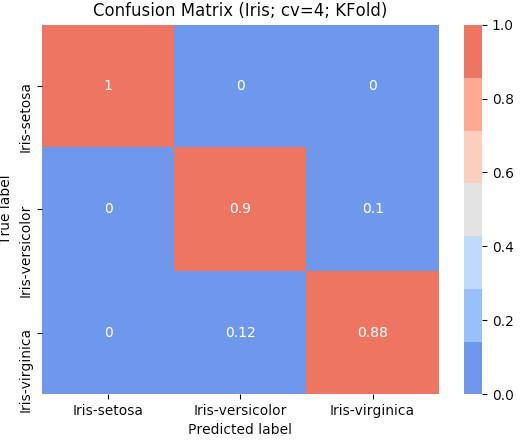
\includegraphics[width=0.7\textwidth]{img/sample_conf_matrix.png}
        \caption{Przykładowa (znormalizowana) macierz konfuzji.}
    \end{figure}